A continuació adjuntarem els diagrames de seqüència corresponents a les operacions de la capa de domini dels casos d'ús de la pràctica.

% LOGIN
\subsection{Login}
\texttt{\textbf{context} CapaDomini :: Login(userN: String, passwd: String)}\\
Aquesta operació rep dos strings: el nom d'usuari i la contrassenya. La comprovació de la excepció \texttt{usernameNoExsiteix} està implícita en el \texttt{get} a la interfície de dades dels usuaris registrats.\\

    %imatge login
    \begin{figure}[h]
    \centering
    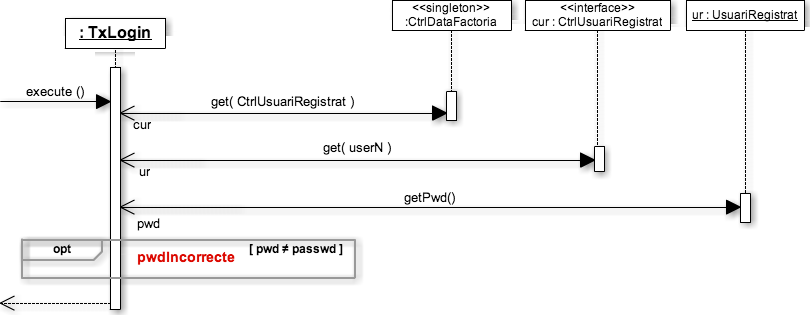
\includegraphics[width=0.6\textwidth]{figures/login.png}
    \caption{Diagrama de seqüència de la operació \texttt{Login}}
    \end{figure}

% CONSULTAR CATEGORIES
\subsection{Consultar Categories}
\texttt{\textbf{context} CapaDomini :: ConsultarCategories(): Set(nom: String)}\\
Aquesta operació retorna un conjunt d'strings amb el nom de totes les categories enregistrades. En el cas que el sistema no disposi de categories, llençarà l'excepció \texttt{noHiHaCategories}.\\

    %imatge consultarCategories
    \begin{figure}[h]
    \centering
    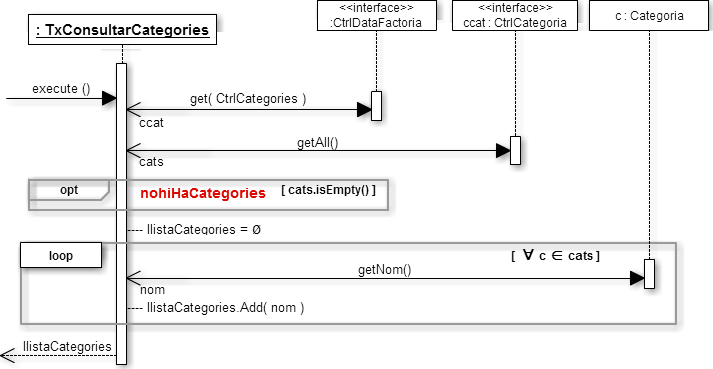
\includegraphics[width=0.6\textwidth]{figures/consultarCategories.png}
    \caption{Diagrama de seqüència de la operació \texttt{ConsultarCategories}}
    \end{figure}

% JUGAR PARTIDA
\subsection{Jugar Partida}
Aquest cas d'ús l'implementem mitjançant un controlador de cas d'ús i conté les següents operacions:


% FER AUTENTIFICACIO
\subsubsection{Fer Autenticació}
\texttt{\textbf{context} CapaDomini :: FerAutenticació(userN: String, passwd: String)}\\
El primer que es fa en aquest cas d'ús és autentificar a l'usuari. Aquest contracte se serveix del cas d'ús anterior (Login): primer s'executa la transacció del login per comprovar que l'usuari existeix i que les dades són correctes i, per acabar, es comprova que l'usuari en qüestió sigui un Jugador i no un Administrador.\\

    %imatge ferAutentificacio
    \begin{figure}[h]
    \centering
    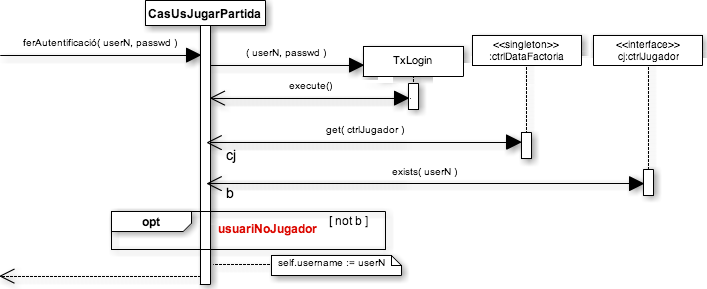
\includegraphics[width=0.7\textwidth]{figures/ferAutentificacio.png}
    \caption{Diagrama de seqüència de la operació \texttt{FerAutentificació}}
    \end{figure}

% OBTENIR CATEGORIES
\subsubsection{Obtenir Categories}
\texttt{\textbf{context} CapaDomini :: ObtenirCategories(): Set(nom: String)}\\
L'únic que fa aquesta operació és cridar al controlador de transacció definit anteriorment, que retorna un conjunt amb els noms de totes les categories del sistema.\\

    %imatge obtenirCategories
    \begin{figure}[h]
    \centering
    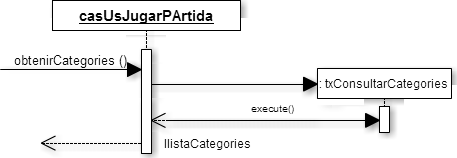
\includegraphics[width=0.6\textwidth]{figures/obtenirCategories.png}
    \caption{Diagrama de seqüència de la operació \texttt{ObtenirCategories}}
    \end{figure}


% CREAR PARTIDA
\subsubsection{Crear Partida}
\small{\texttt{\textbf{context} CapaDomini :: CrearPartida(cat: String): TupleType(puntuacióInicial: Integer, nombreMàximErrors: Integer, puntuacióPerEncert: Integer, puntuacióPerError: Integer[0..1])
}}\\
Aquesta operació obté en primer lloc totes les dades que necessita per a crear una partida. Després crida a una operació que crea el tipus d'estratègia que se li assignarà a la partida en funció del nombre de partides guanyades del jugador. Una vegadarecopilada tota la informació, crea la partida, que s'associa amb el jugador, l'estratègia i la paraula corresponent, i també es creen totes les caselles.\\

    %imatge crearPartida
    \begin{figure}[h!]
    \centering
    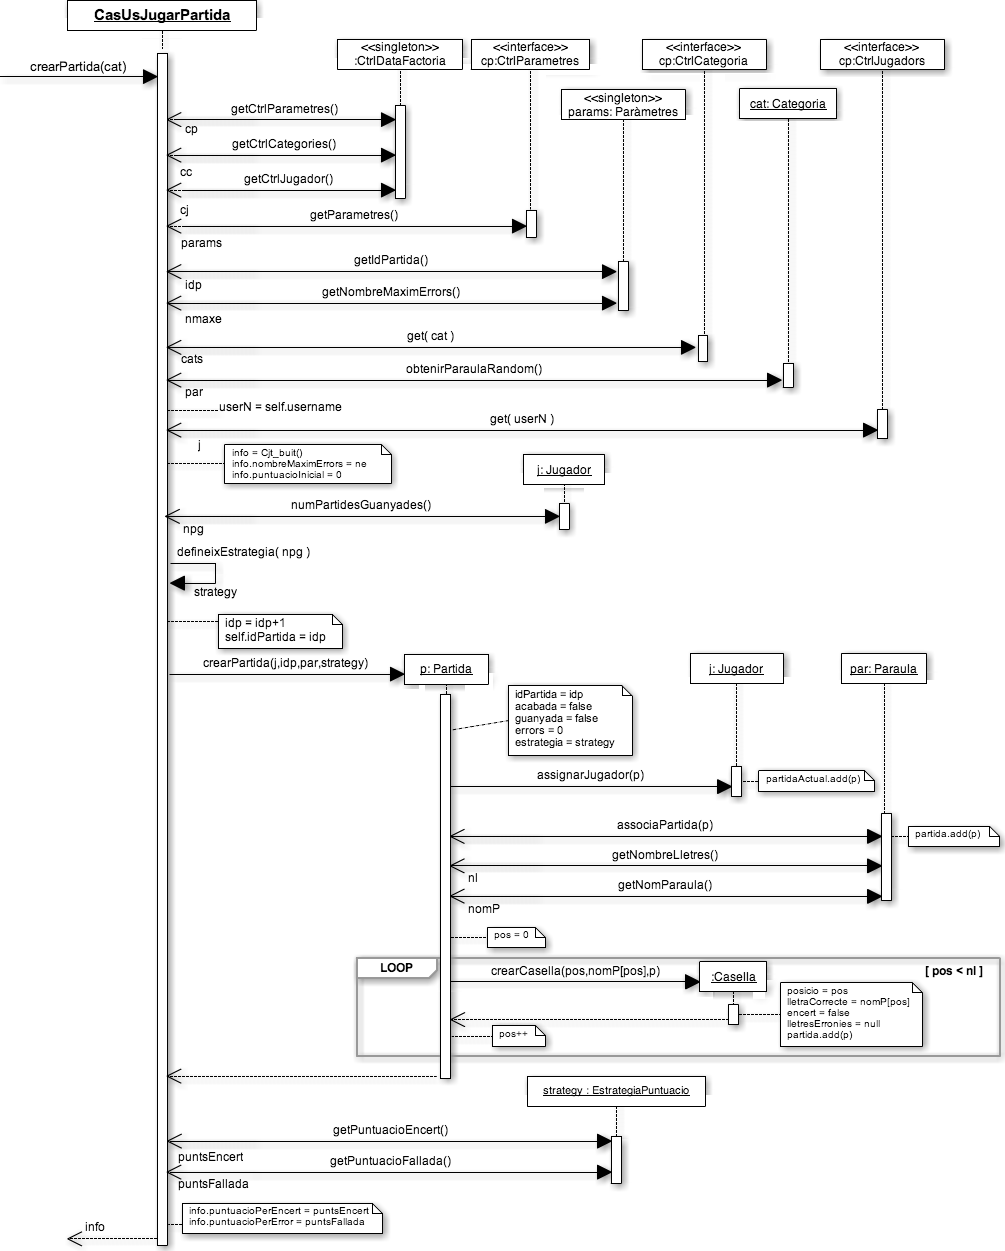
\includegraphics[width=0.8\textwidth]{figures/crearPartida.png}
    \caption{Diagrama de seqüència de la operació \texttt{CrearPartida}}
    \end{figure}


    %imatge opsCrearPartida
    \begin{figure}[h]
    \centering
    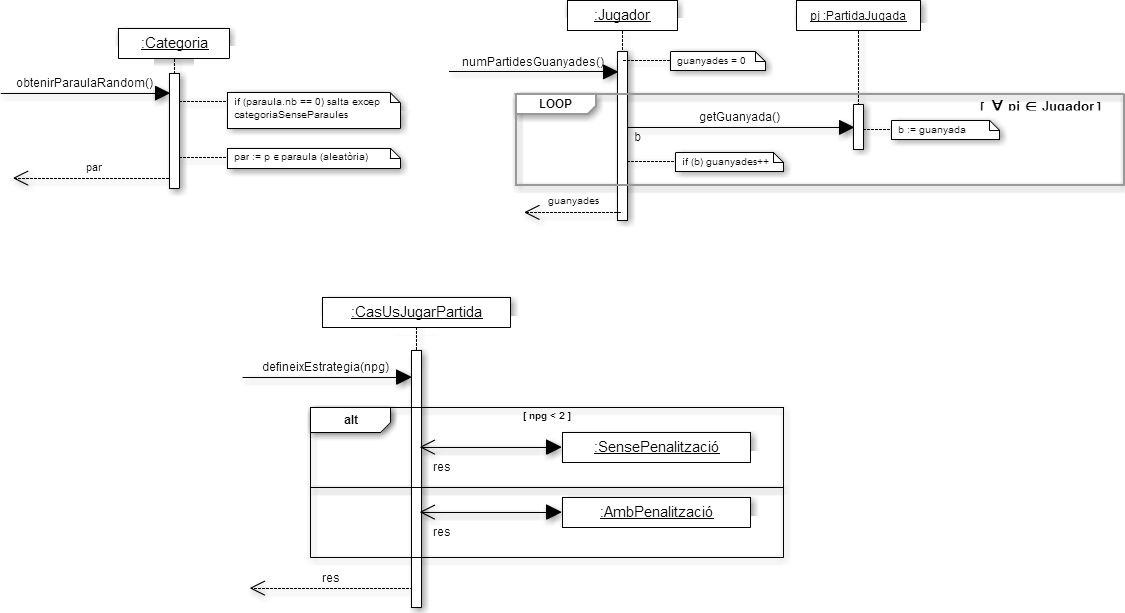
\includegraphics[width=0.8\textwidth]{figures/opsCrearPartida.png}
    \caption{Diagrama de seqüència de les operacions auxiliars de \texttt{CrearPartida}}
    \end{figure}

% FER JUGADA
\subsubsection{Fer Jugada}
\small{\texttt{\textbf{context} CapaDomini :: FerJugada(pos: Integer, lletra: String): TupleType( encert: Boolean, acabada: Boolean, guanyada: Boolean, puntuació: Integer, errors: Integer)}} \\
A \texttt{FerJugada} primer es comprova que la lletra entrada és una opció vàlida, i llavors es crida a una operació de la classe \texttt{Partida} que serà la que actualitzarà tot el que calgui i ens tornarà la tupla amb la informació que volem.\\
Aquest \texttt{ferJugada} de \texttt{Partida} actulitza primer l'estat de la casella que toqui i després calcula la puntació en funció de l'estratègia definida. En el cas que es produeixi un encert, es comprova si s'ha guanyat la partida i s'envia un missatge al jugador mitjançant el servei de missatgeria. Per acabar, es mira si la partda s'ha acabat, per tal d'actualitzar les associacions amb \texttt{Jugador}.

    %imatge fer jugada 1
    \begin{figure}[h]
    \centering
    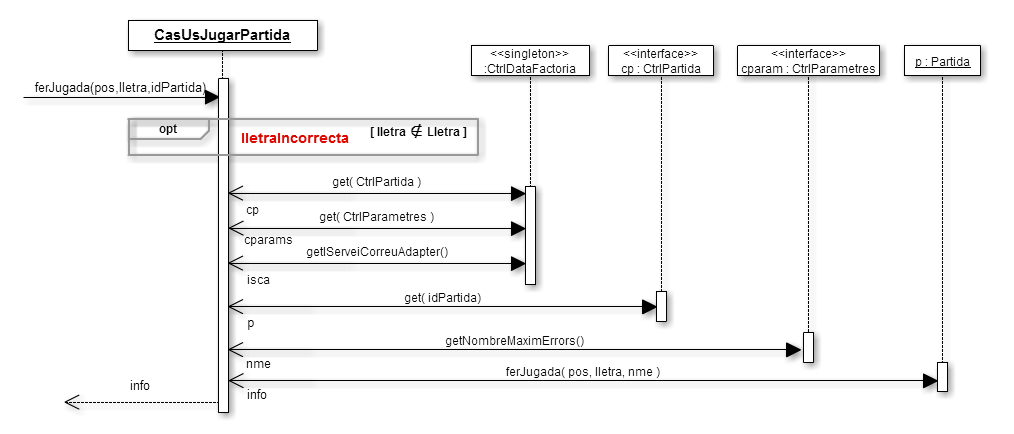
\includegraphics[width=0.8\textwidth]{figures/ferJugada1.png}
    \caption{Diagrama de seqüència de la operació \texttt{ferJugada}}
    \end{figure}
    
     %imatge fer jugada 2
    \begin{figure}[h!]
    \centering
    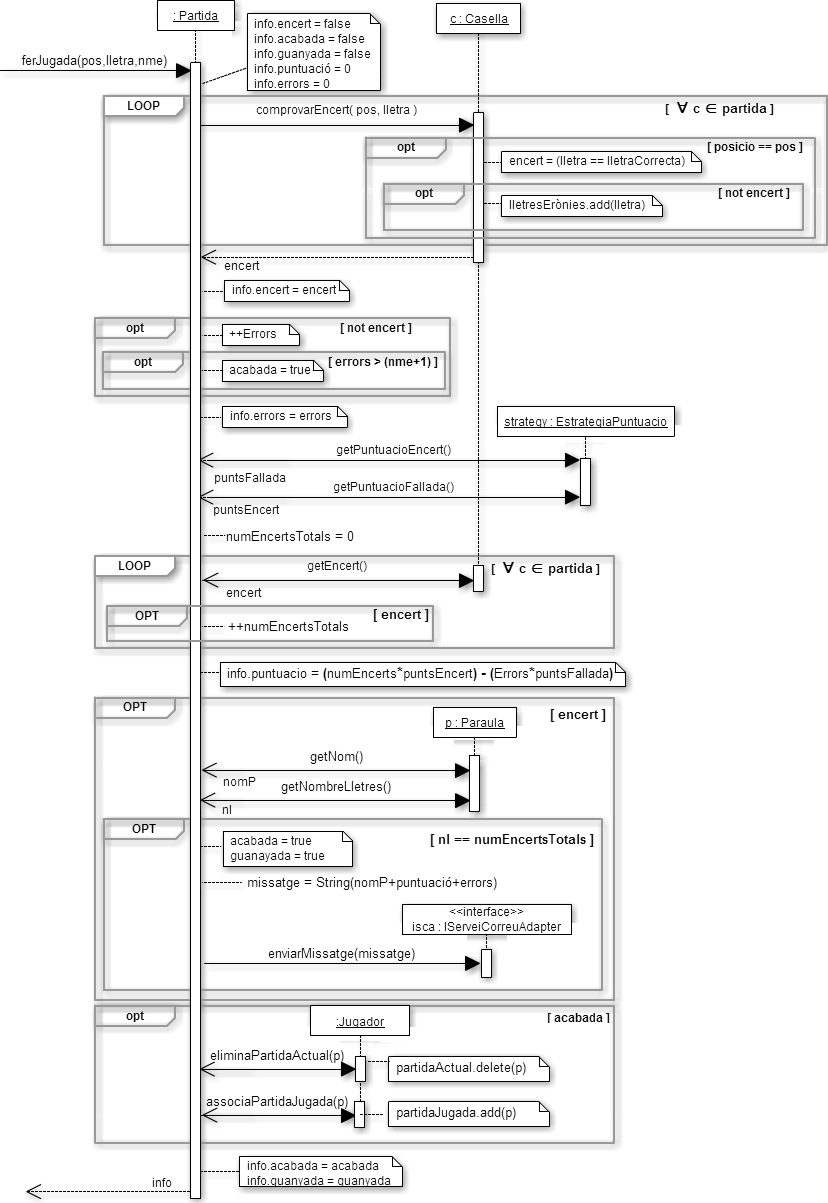
\includegraphics[width=0.9\textwidth]{figures/ferJugadaBe2.png}
    \caption{Diagrama de seqüència de la operació \texttt{ferJugada} de la classe Partida}
    \end{figure}

  %imatge ops fer jugada 
    \begin{figure}[h!]
    \centering
    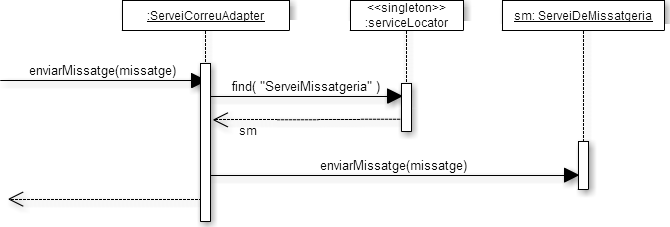
\includegraphics[width=0.8\textwidth]{figures/opsFerJugada.png}
    \caption{Diagrama de seqüència de les operacions auxiliars de \texttt{ferJugada}}
    \end{figure}
    
% ATURAR PARTIDA
\subsubsection{Aturar Partida}
\texttt{\textbf{context} CapaDomini :: aturarParida()}\\
Aquesta operació esborra l'associació de \texttt{Jugador} amb el rol \texttt{partidaActual}, i en crea una amb el rol \texttt{partidaJugada}.\\

    %imatge atuurarPartida
    \begin{figure}[h]
    \centering
    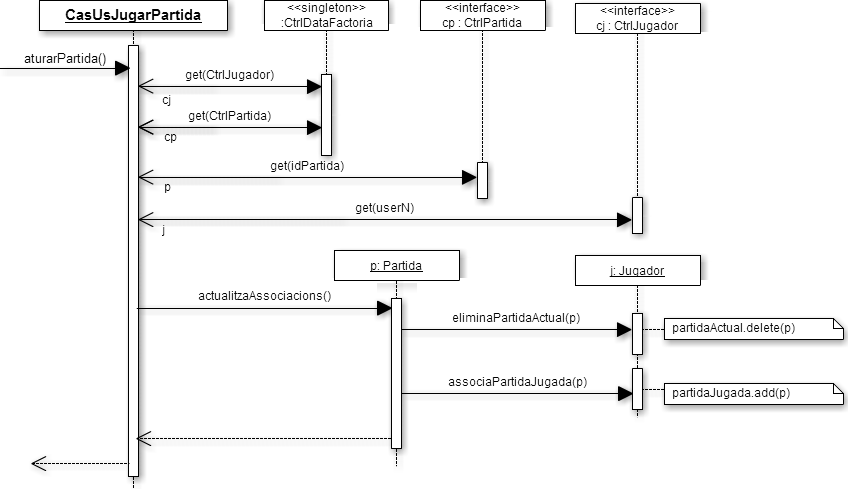
\includegraphics[width=0.8\textwidth]{figures/aturarPartida.png}
     \caption{Diagrama de seqüència de la operació \texttt{aturarPartida}}
    \end{figure}
